\setbeamertemplate{caption}{\raggedright\insertcaption\par}
\subsubsection{CAD input files}
\begin{frame}{CAD input files}

%Red faces (RGB=[255,0,0]): Fixture
%\item Green faces (RGB=[0,255,0]): Non-changing region  
%\item Colored (RGB=[0-255,0-255,0-255]): 3D loading vector 
%Linear force scaling: $F=f*({\bf x}-127)$\\
%One Byte: 0-126 negative, 127 zero, 128-255 positive direction
\begin{figure}
\centering
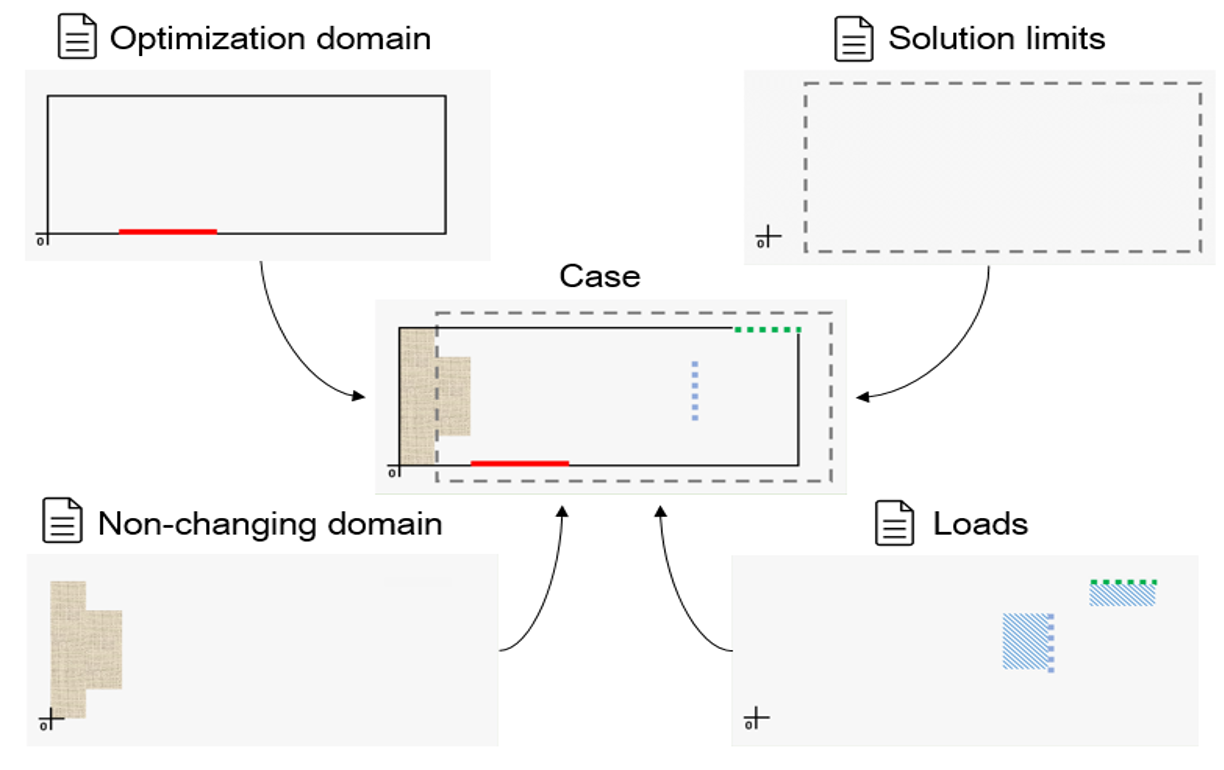
\includegraphics[width=.84\textwidth]{Pictures/SecondHalf/four_files.png}
\end{figure}
\end{frame}

\subsubsection{Voxelization}
\begin{frame}{Voxelized geometry}
\begin{itemize}
\item Done using OpenCascade  
\item Each region voxelized separately 
\end{itemize}
\vspace{0.4cm}
%\begin{enumerate}
%\item Active voxels (geometry)
%\item Fixture voxels
%\item Non-changing voxels
%\item Load voxels
%\end{enumerate}
\begin{minipage}{0.49\textwidth}
\begin{figure}
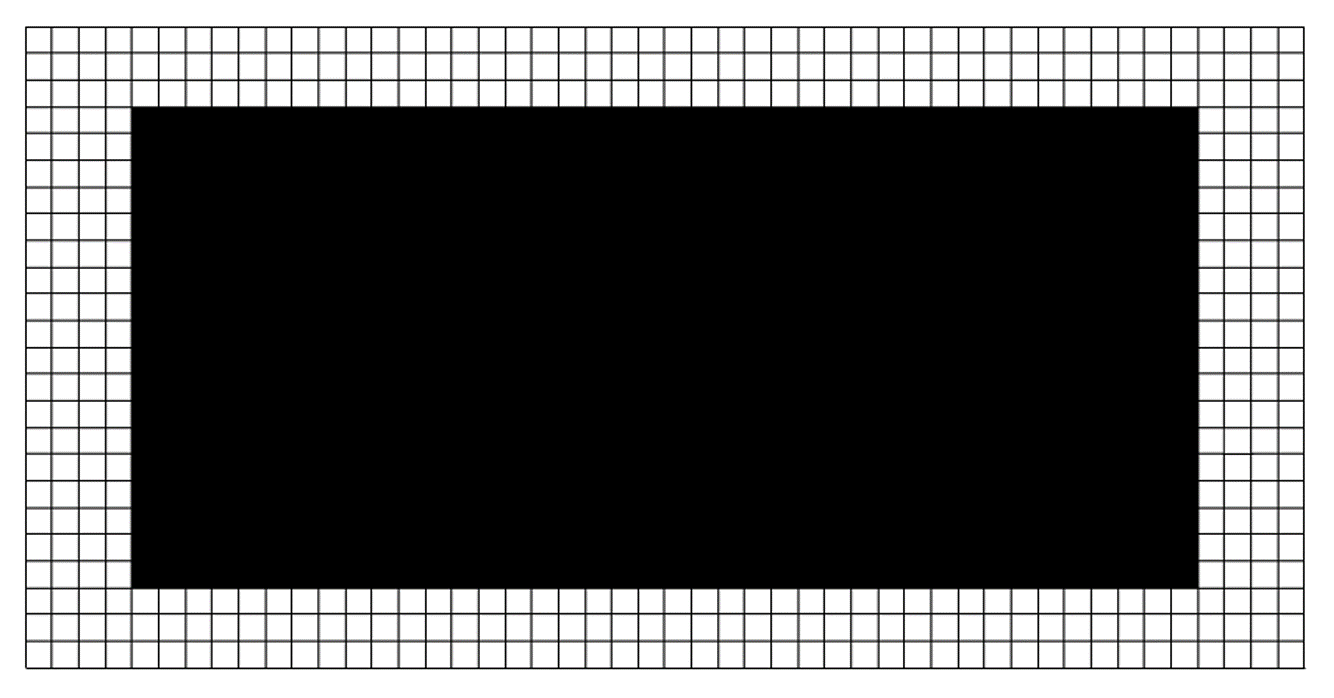
\includegraphics[width=.8\textwidth]{Pictures/Voxels/Active_2.png}
\caption{Participating voxels}
\end{figure}
\vspace{-0.6cm}
 \begin{figure}
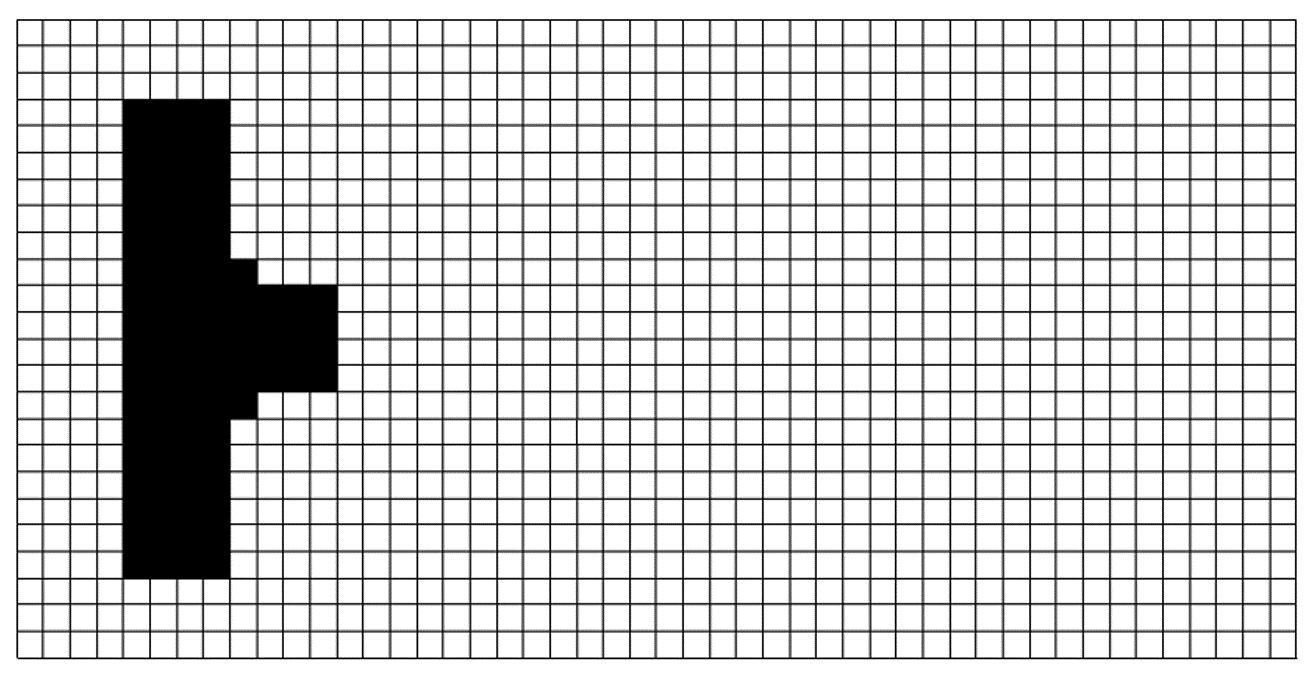
\includegraphics[width=.8\textwidth]{Pictures/Voxels/NonChanging.png}
\caption{Non-Changing Voxels}
\end{figure}
\end{minipage}
\hfill
\begin{minipage}{0.49\textwidth}
\begin{figure}
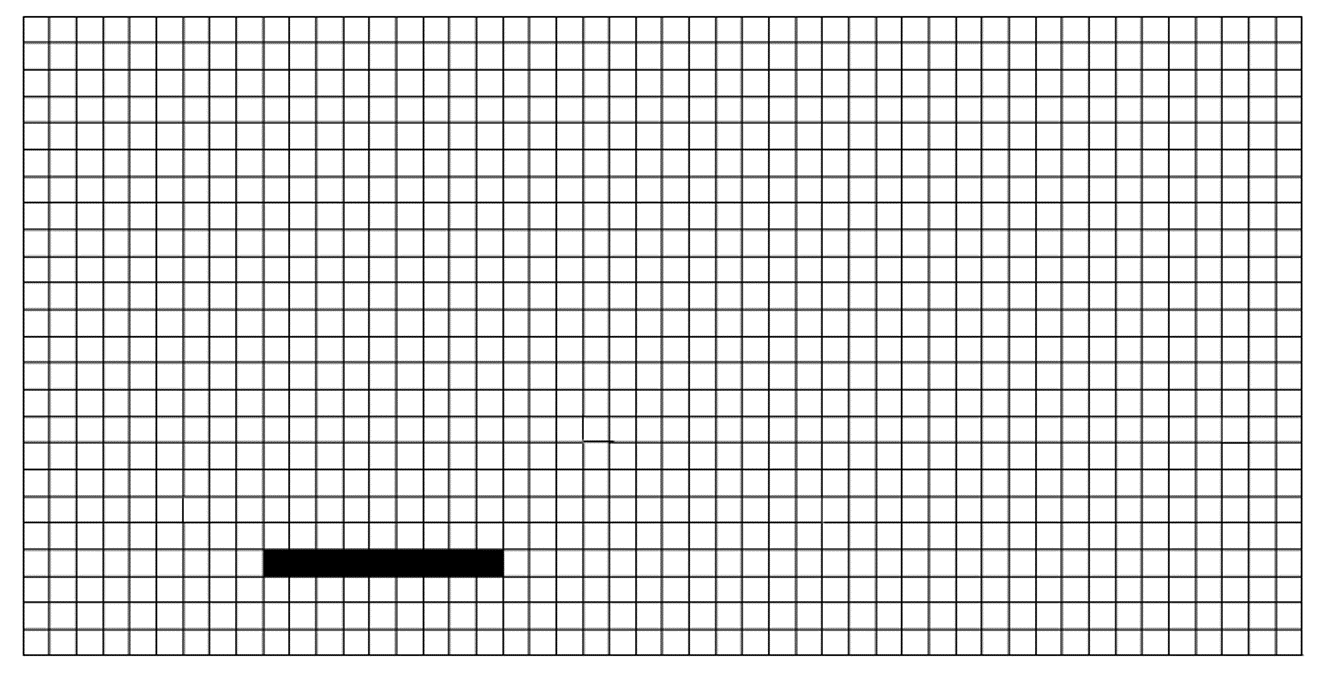
\includegraphics[width=.8\textwidth]{Pictures/Voxels/Fixture.png}
\caption{Fixture voxels}
\end{figure}
\vspace{-0.6cm}
\begin{figure}
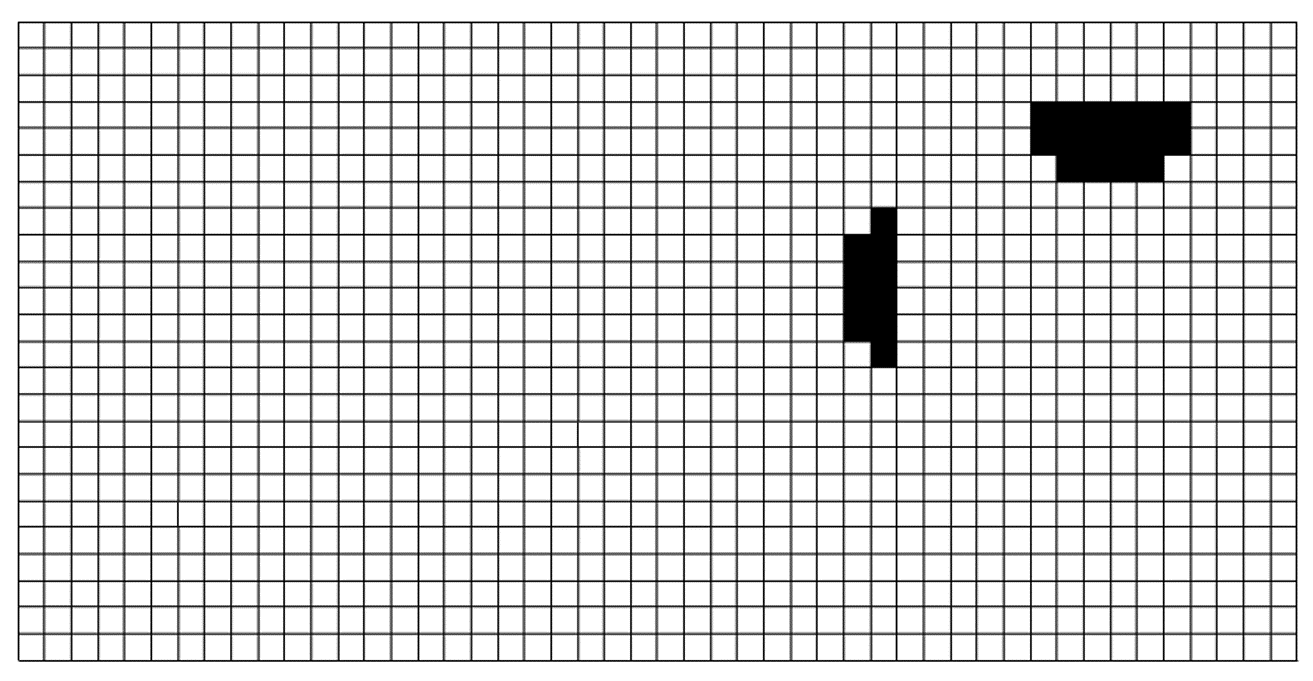
\includegraphics[width=.8\textwidth]{Pictures/Voxels/Load.png}
\caption{Load voxels}
\end{figure}
\end{minipage}
\end{frame}

\subsubsection{Black-Box Topology Optimizer}
\begin{frame}{Topology Optimization Process}
\begin{overlayarea}{\textwidth}{.9\textheight}
\begin{tikzpicture} [remember picture,overlay]
		\uncover<1->{
		\node[anchor=north,inner sep=0pt] [xshift=5cm,yshift=-0cm] (N1)
                {Provide geometry as voxel grid};
		}     
        \uncover<2->{
        \node [below =of N1, inner sep=0pt](N2){Calculate stress on each voxel};
        \draw[thick,->] (N1) -- (N2);
		}
		\uncover<3->{
		\node [right =of N2, xshift=2.5cm, inner sep=0pt](N3){};
		\node [below =of N3, yshift=-4cm, inner sep=0pt](N4){};
		\node [left =of N4, xshift=-2.0cm, inner sep=0pt](N5){If stress below threshold, remove voxel};
        \draw[thick,->] (N2) -- (N3) -- (N4) -- (N5);
		}
		\uncover<4->{
		\node [left =of N5, xshift=-1.3cm, inner sep=0pt](N6){};
		\node [left =of N2, xshift=-2cm, inner sep=0pt](N7){};
        \draw[thick,->] (N5) -- (N6) -- (N7) -- (N2);
		}
		\uncover<5->{
			\only<5>{
			\node [below =of N2, xshift=0.5cm, yshift=1cm](Picture){
				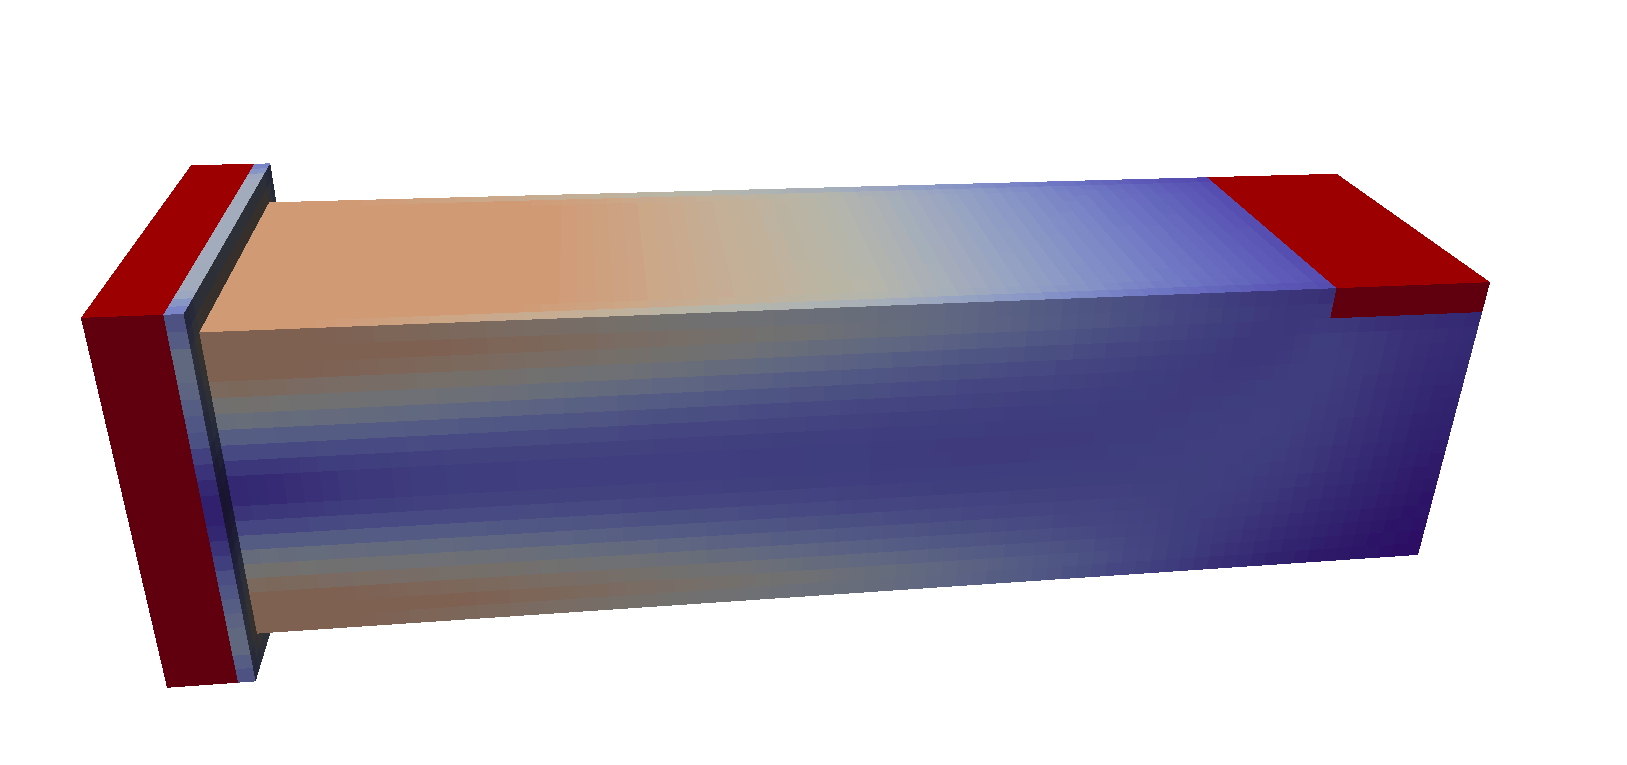
\includegraphics[scale=0.15]{Pictures/SecondHalf/Topology/Cantilever_Topy_0.png}
				};
			}	
			\only<6>{
			\node [below =of N2, xshift=0.5cm, yshift=1cm](Picture){
				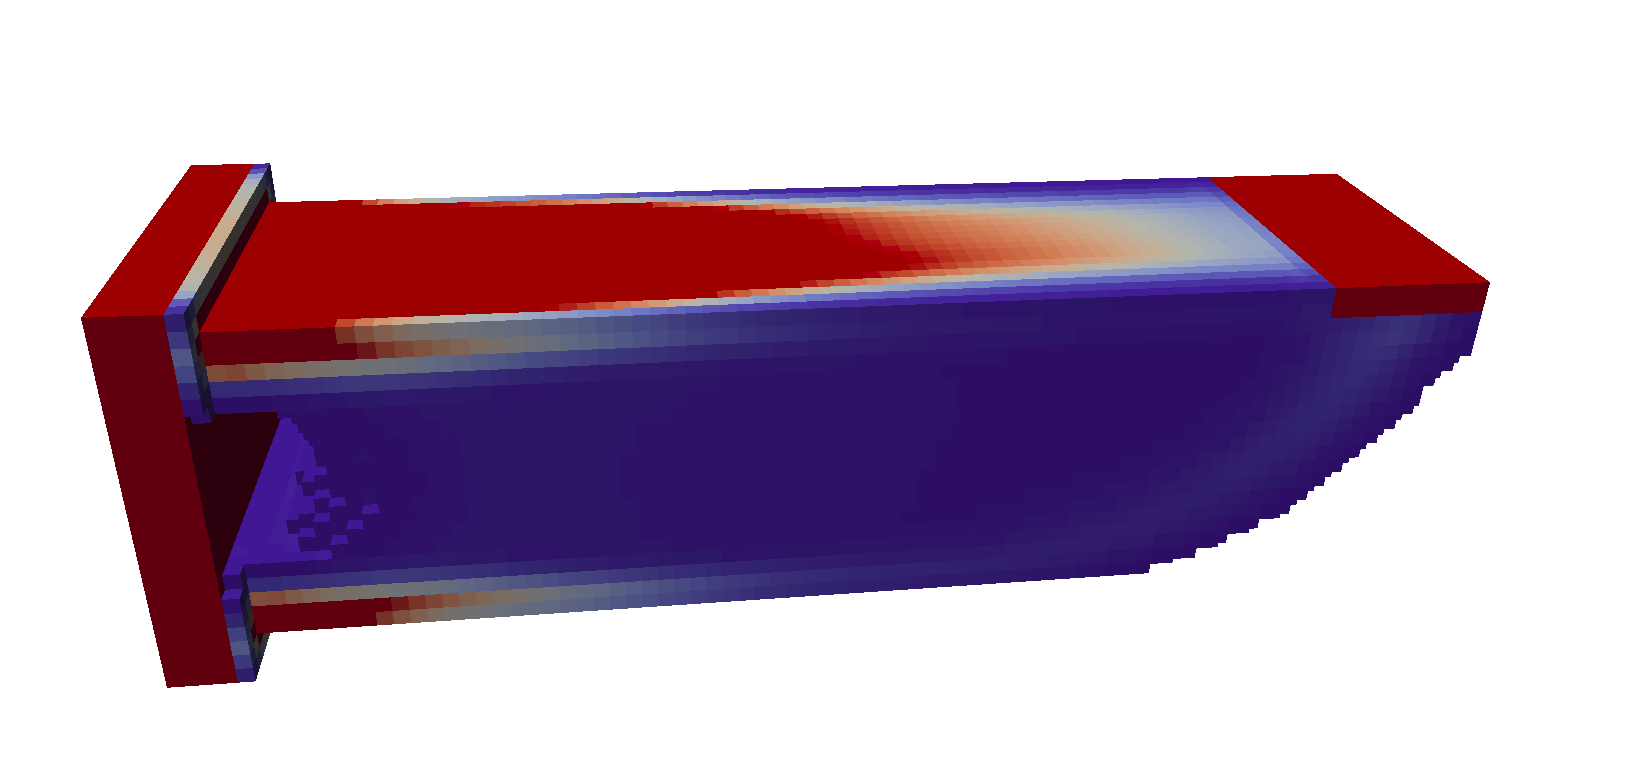
\includegraphics[scale=0.15]{Pictures/SecondHalf/Topology/Cantilever_Topy_1.png}
				};
			}	
			\only<7>{
			\node [below =of N2, xshift=0.5cm, yshift=1cm](Picture){
				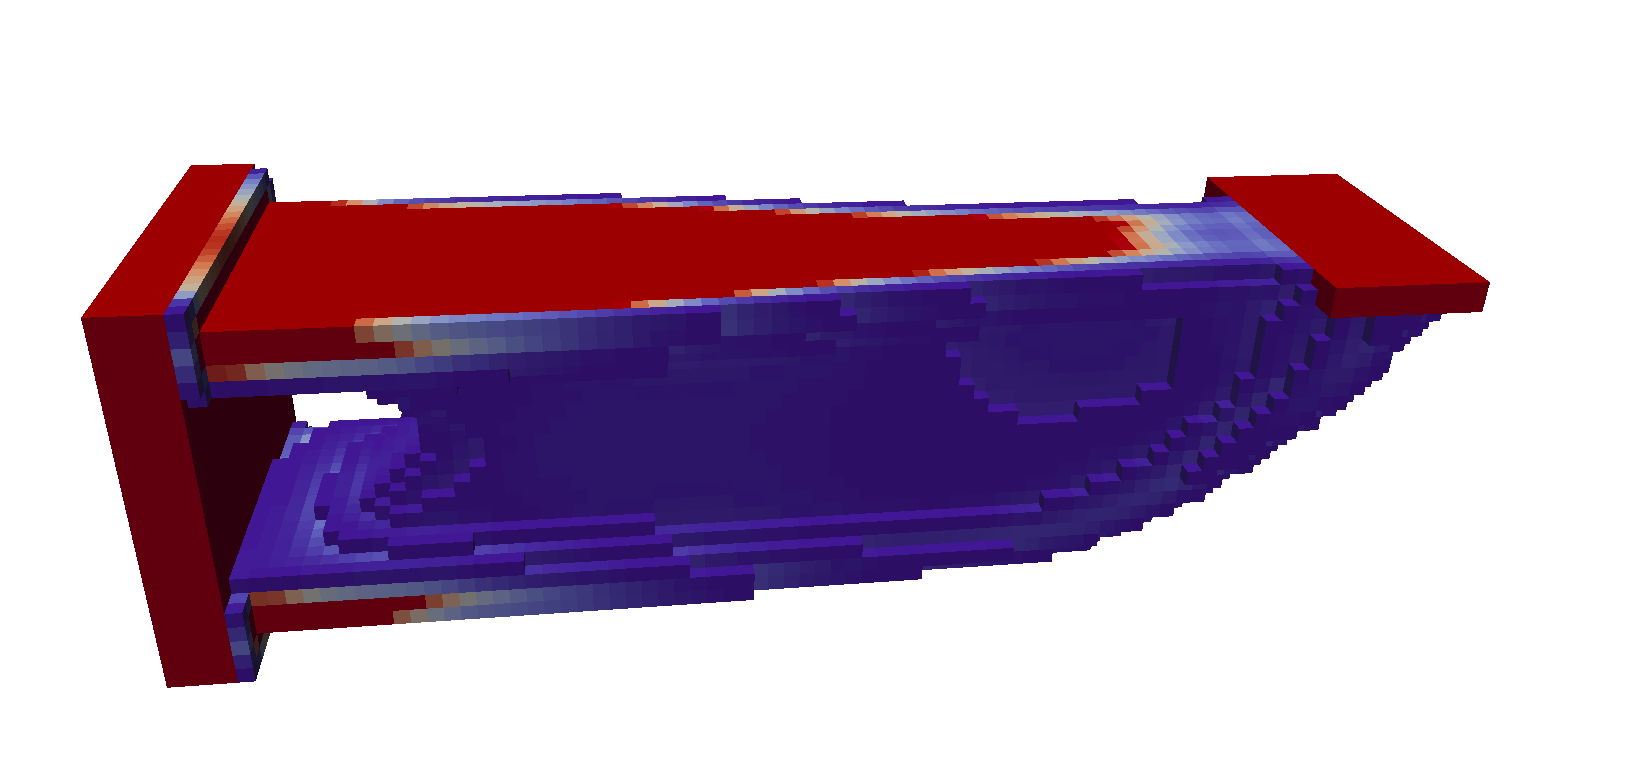
\includegraphics[scale=0.15]{Pictures/SecondHalf/Topology/Cantilever_Topy_2.png}
				};
			}	
			\only<8>{
			\node [below =of N2, xshift=0.5cm, yshift=1cm](Picture){
				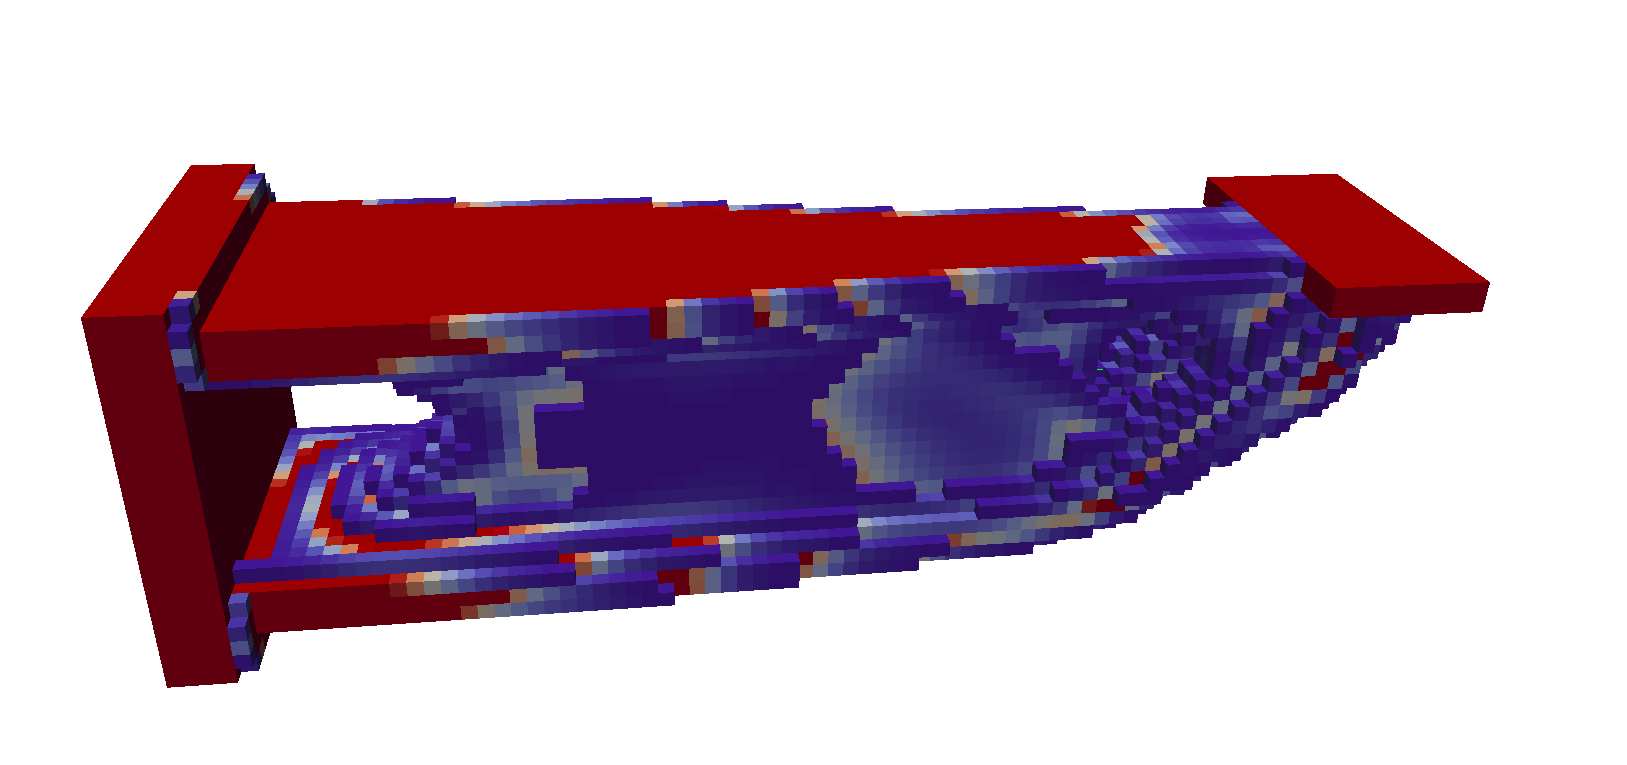
\includegraphics[scale=0.15]{Pictures/SecondHalf/Topology/Cantilever_Topy_3.png}
				};
			}	
			\only<9>{
			\node [below =of N2, xshift=0.5cm, yshift=1cm](Picture){
				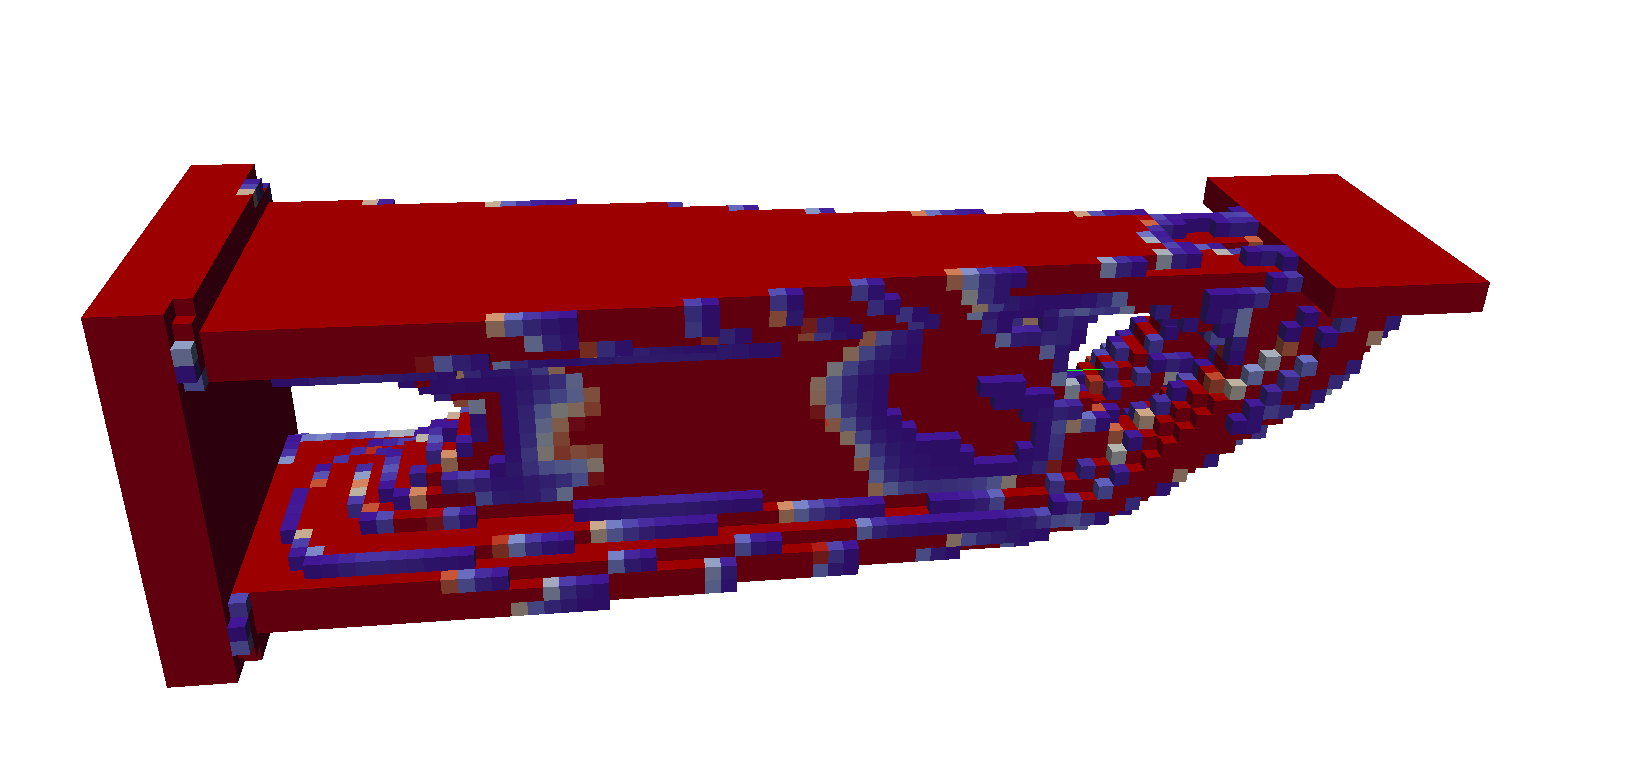
\includegraphics[scale=0.15]{Pictures/SecondHalf/Topology/Cantilever_Topy_4.png}
				};
			}	
			\only<10>{
			\node [below =of N2, xshift=0.5cm, yshift=1cm](Picture){
				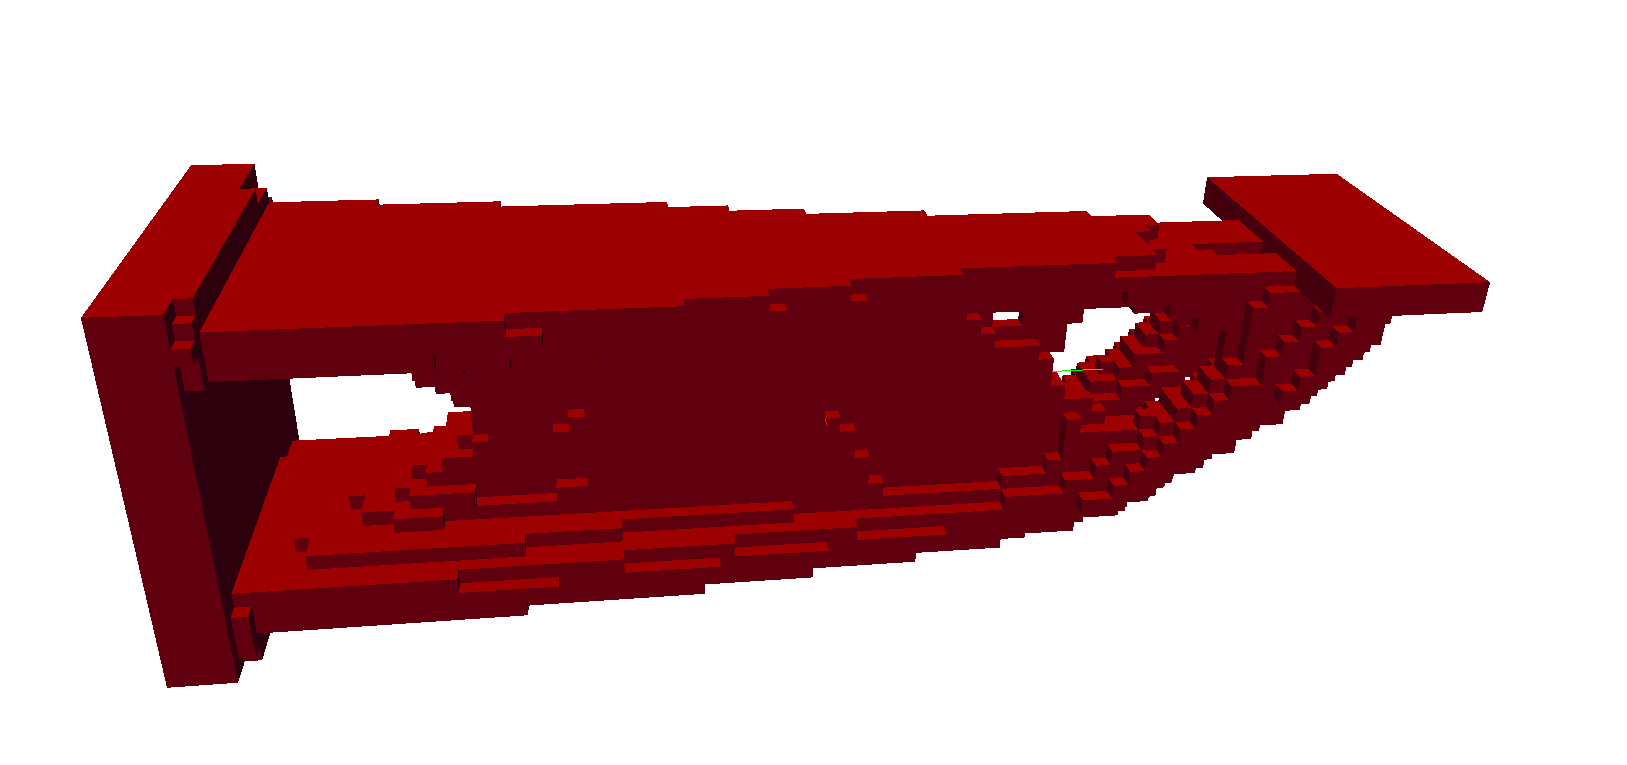
\includegraphics[scale=0.15]{Pictures/SecondHalf/Topology/Cantilever_Topy_5.png}
				};
			}	
		}
\end{tikzpicture}
\end{overlayarea}
\end{frame}

%\begin{frame}{Topology Optimization Process}
%\begin{center}
%Provide geometry as voxel grid
%$$\downarrow$$
%Calculate stress on each voxel
%$$\downarrow$$
%Remove voxel from active geometry if stress is below threshold
%\end{center}
%\end{frame}
%
%\begin{frame}{Topology Optimization Example}
%\only<1>{
%\begin{figure}
%\centering
%%\vspace{-0.5cm}
%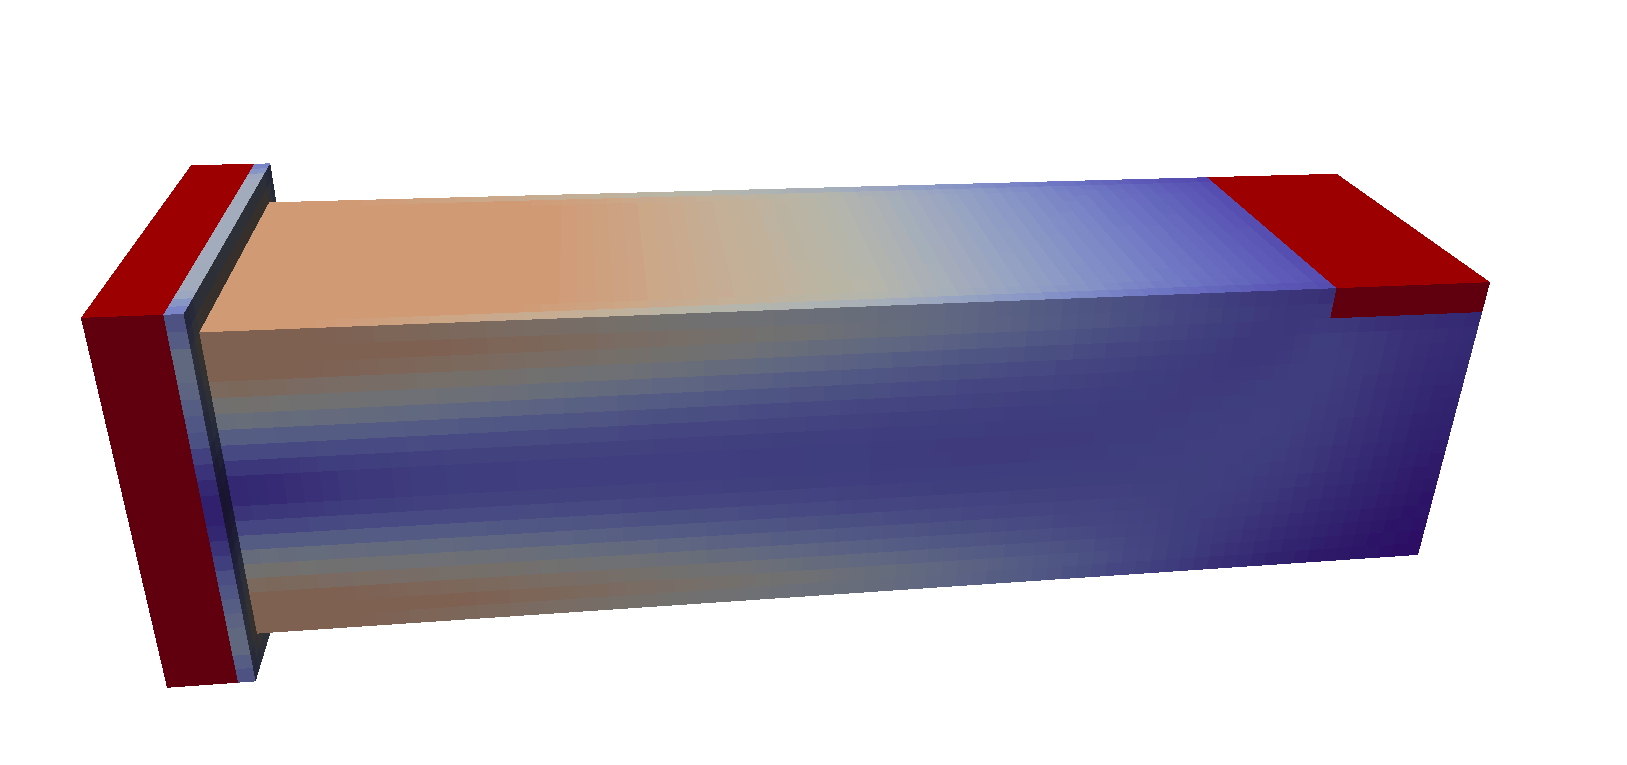
\includegraphics[width=1\textwidth]{Pictures/SecondHalf/Topology/Cantilever_Topy_0.png}
%\end{figure}}
%\only<2>{
%\begin{figure}
%\centering
%%\vspace{-0.5cm}
%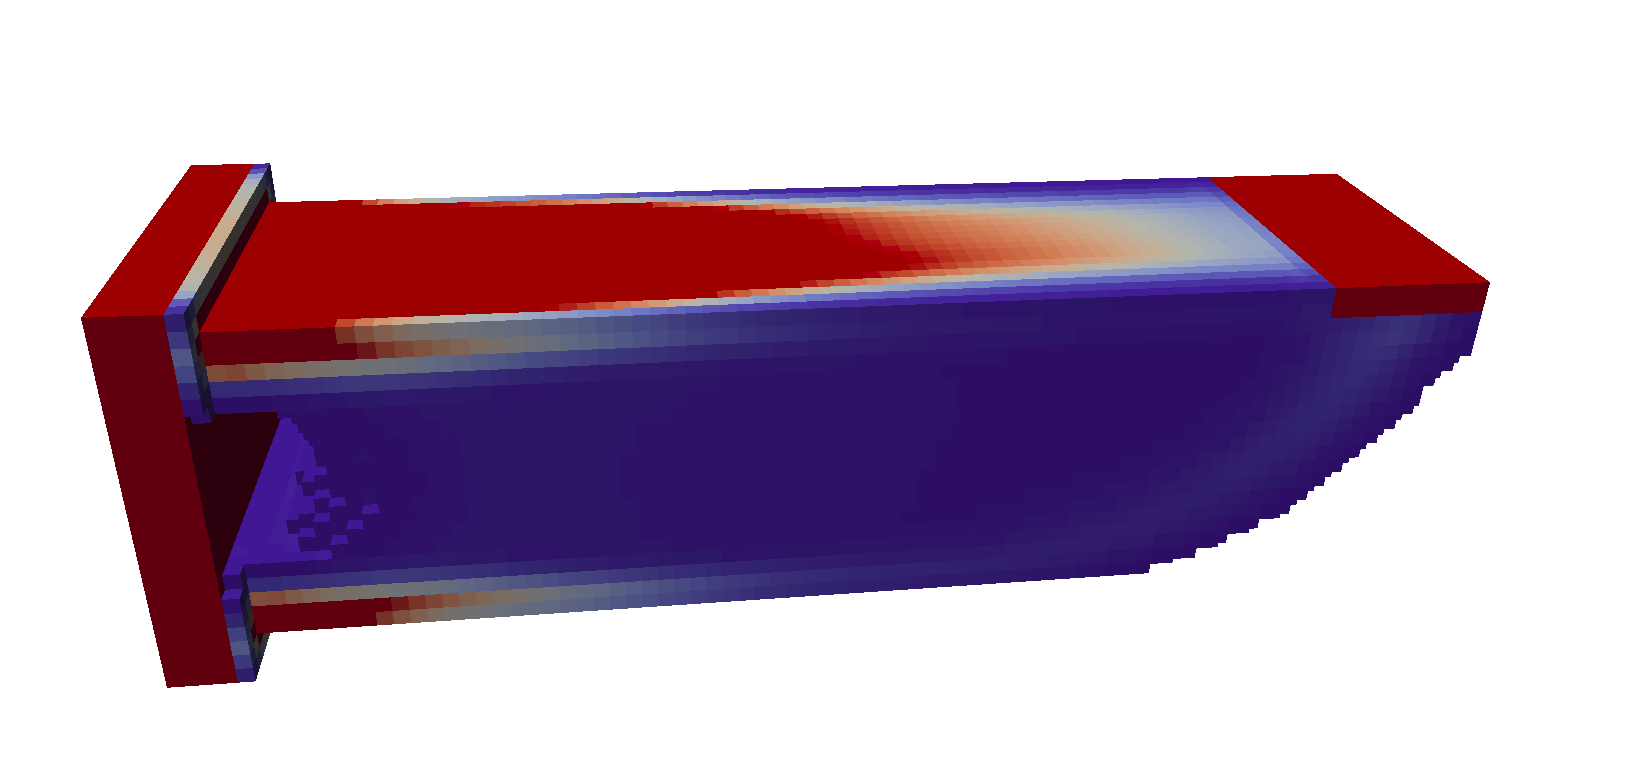
\includegraphics[width=1\textwidth]{Pictures/SecondHalf/Topology/Cantilever_Topy_1.png}
%\end{figure}}
%\only<3>{
%\begin{figure}
%\centering
%%\vspace{-0.5cm}
%\includegraphics[width=1\textwidth]
%{Pictures/SecondHalf/Topology/Cantilever_Topy_2.png}
%\end{figure}}
%\only<4>{
%\begin{figure}
%\centering
%%\vspace{-0.5cm}
%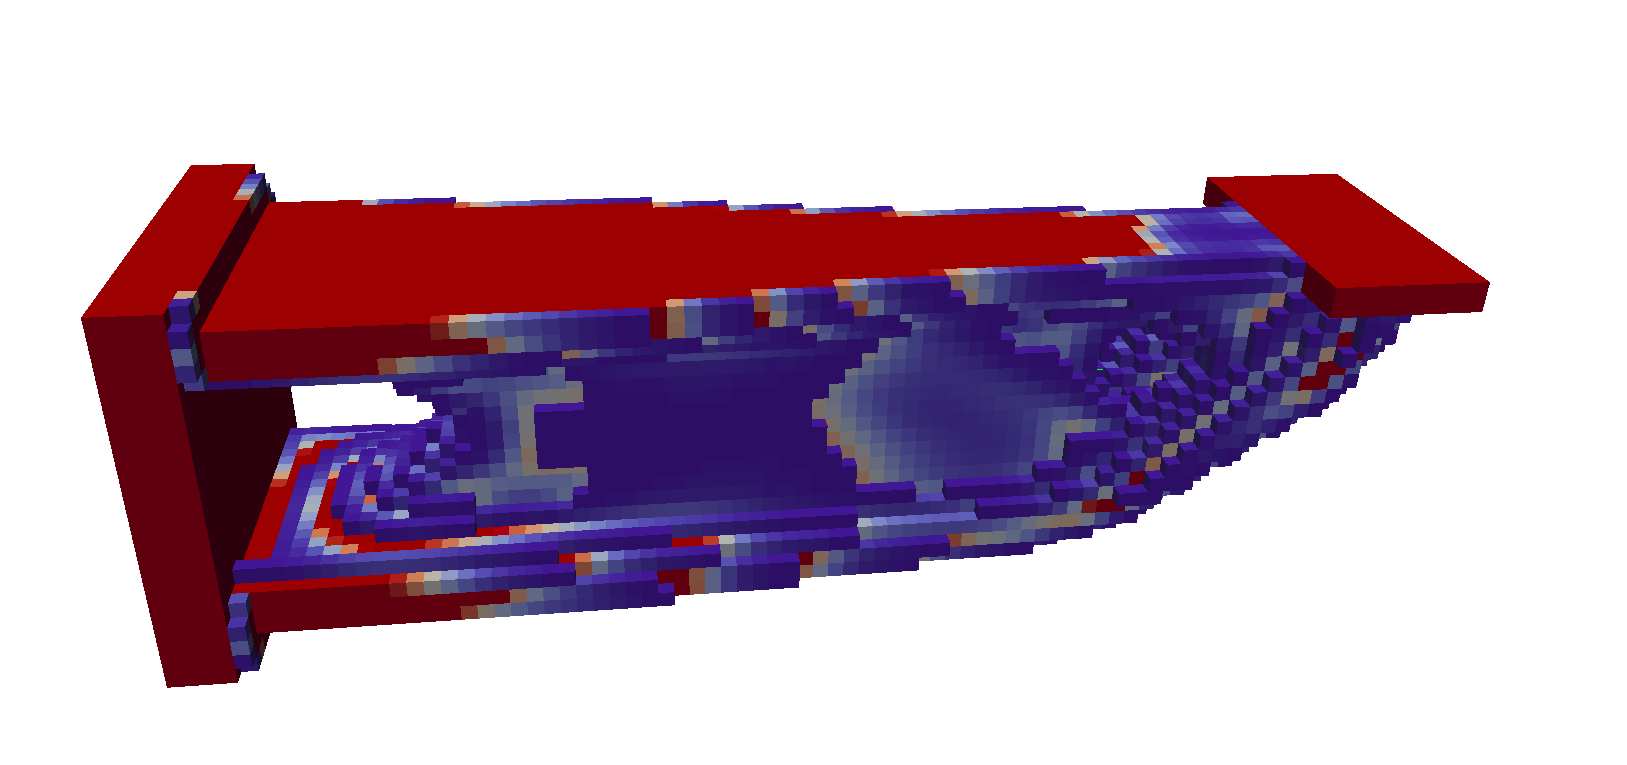
\includegraphics[width=1\textwidth]{Pictures/SecondHalf/Topology/Cantilever_Topy_3.png}
%\end{figure}}
%\only<5>{
%\begin{figure}
%\centering
%%\vspace{-0.5cm}
%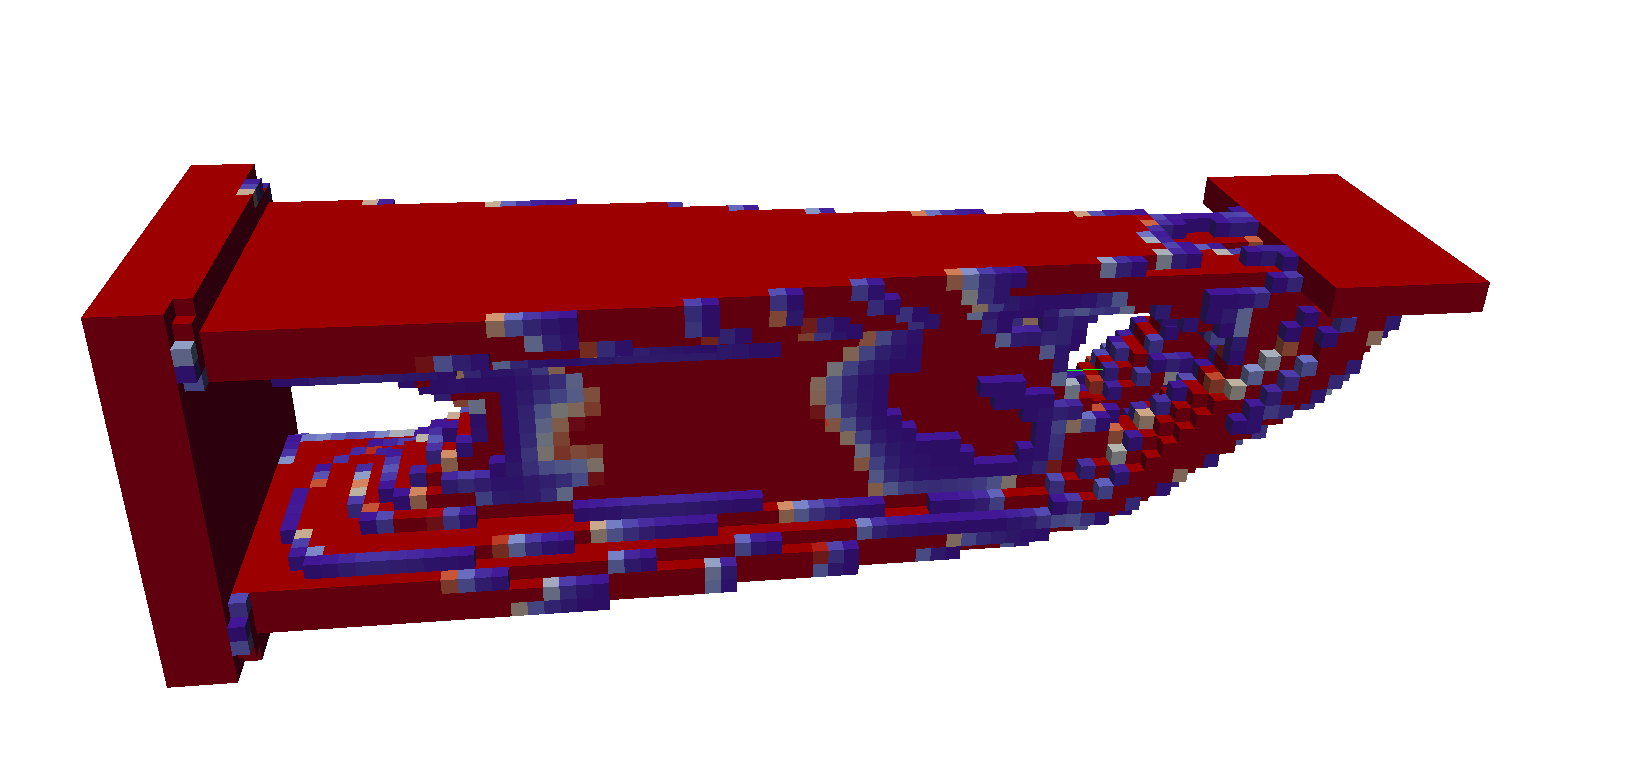
\includegraphics[width=1\textwidth]{Pictures/SecondHalf/Topology/Cantilever_Topy_4.png}
%\end{figure}}
%\only<6>{
%\begin{figure}
%\centering
%%\vspace{-0.5cm}
%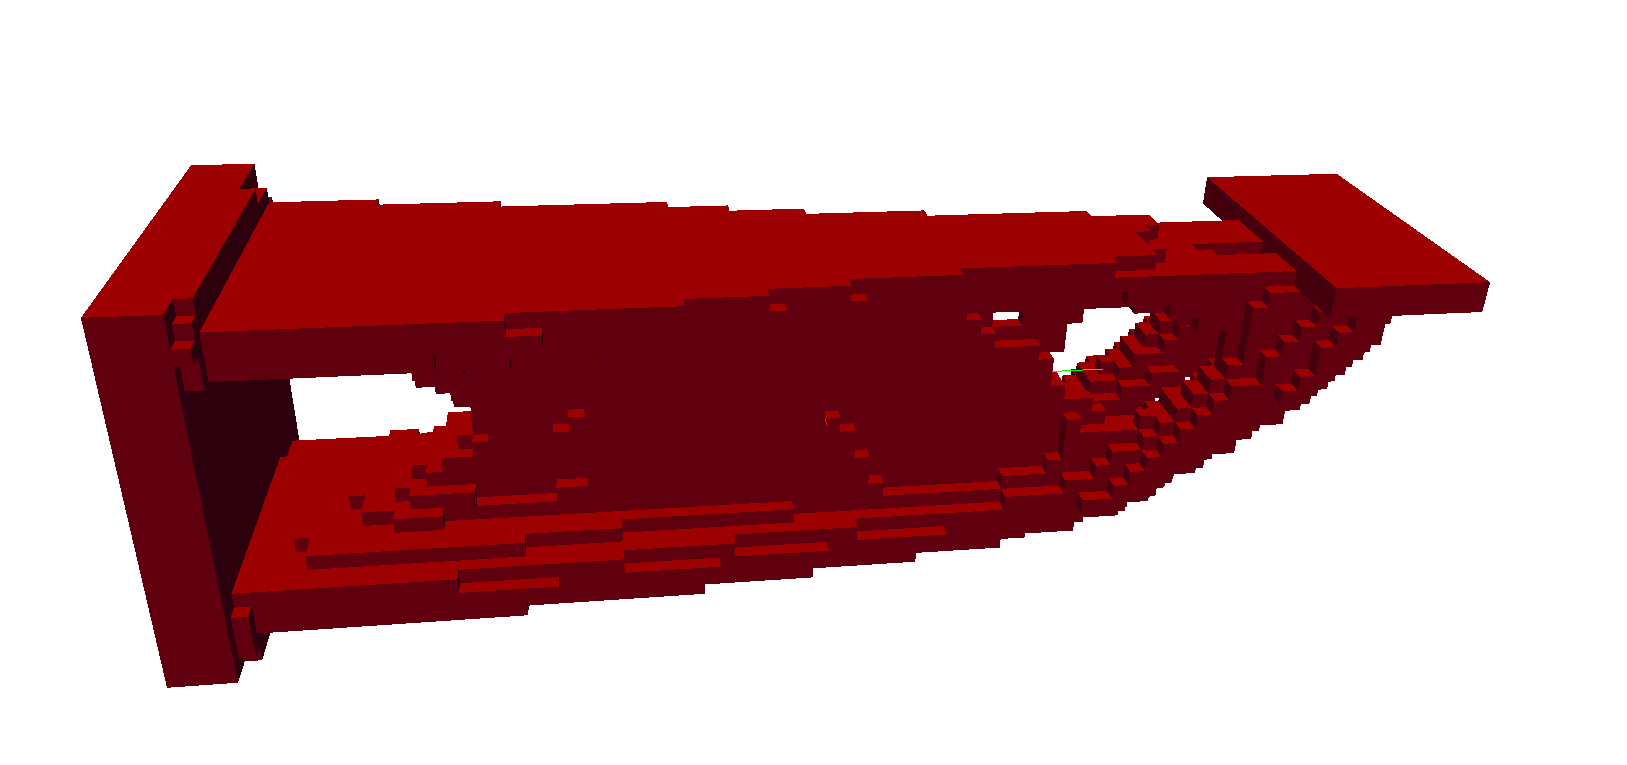
\includegraphics[width=1\textwidth]{Pictures/SecondHalf/Topology/Cantilever_Topy_5.png}
%\end{figure}}
%\end{frame}
